\documentclass[
  11pt,
  letterpaper,
   addpoints,
   answers
  ]{exam}

\usepackage[utf8]{inputenc}
\usepackage{../exercise-preamble}
\usepackage{float}
\usepackage{subcaption}
\usepackage{pgfplots}
\pgfplotsset{compat=1.18}
\usepgfplotslibrary{groupplots}
% TikZ libraries needed for `right=.. of ..` and coordinate math
\usetikzlibrary{positioning,calc,arrows,arrows.meta}

% Configuración de numeración de páginas
\makeatletter
\def\@oddfoot{\hfil Página \thepage \hfil}
\def\@evenfoot{\hfil Página \thepage \hfil}
\def\@oddhead{}
\def\@evenhead{}
\makeatother

\begin{document}

% Configuración del encabezado usando comandos de la clase exam
\pagestyle{headandfoot}
\extraheadheight{0.5in} % Baja el encabezado aumentando el espacio superior
\firstpageheader{\textit{Análisis de señales}}{}{EL3203}
\runningheader{\textit{Análisis de señales}}{}{EL3203}
\firstpagefooter{}{\thepage}{}
\runningfooter{}{\thepage}{}
\headrule % Línea debajo del encabezado

% Numeración de página
\pagenumbering{arabic}

% Portada
\begin{center}
    \vspace*{1cm}
    
    % Logo superior
    \includegraphics[width=0.5\textwidth]{../fcfm_die}
    
    \vspace{2cm}
    
    % Líneas decorativas superiores
    
\begin{tikzpicture}
        \draw[line width=2pt, black!70] (0,0) -- (10,0);
        \draw[line width=0.5pt, black!50] (0,0.2) -- (10,0.2);
    \end{tikzpicture}
    
    \vspace{1cm}
    
    % Título principal
    {\fontsize{28}{34}\selectfont\bfseries 
   Análisis de señales}
    
    \vspace{0.5cm}
    
    {\Large\textbf{EL3203}}
    
    \vspace{1cm}
    
    % Líneas decorativas inferiores
    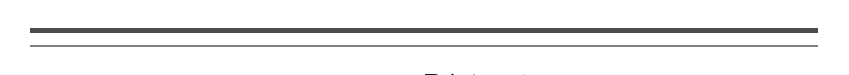
\begin{tikzpicture}
        \draw[line width=0.5pt, black!50] (0,0) -- (10,0);
        \draw[line width=2pt, black!70] (0,0.2) -- (10,0.2);
    \end{tikzpicture}
    
    \vspace{1.5cm}
    
    % Subtítulo
    {\LARGE\itshape Pauta Auxiliar 6 - DFT}
    
    \vspace{0.5cm}
    {\large Prof Jorge Silva.}\\
    {\large Prof Auxiliar Erik Sáez Aravena.}
    
    \vfill
    

    \vspace{1cm}
    
\end{center}

\newpage
%----------------------------
\section{Resumen}

\subsection*{Transformada Discreta de Fourier (DFT): Señales Discretas Periódicas}

La DFT maneja señales discretas y periódicas (o de duración finita), produciendo espectros discretos:

\begin{align}
X[k] &= \sum_{n=0}^{N-1} x[n]\,e^{-j\frac{2\pi kn}{N}} \quad \text{(Análisis)} \tag{DFT}\\
x[n] &= \frac{1}{N}\sum_{k=0}^{N-1} X[k]\,e^{j\frac{2\pi kn}{N}} \quad \text{(Síntesis)} \tag{IDFT}
\end{align}

\subsection*{Propiedades Fundamentales}

\begin{enumerate}
\item \textbf{Linealidad:}
\begin{equation}
ax_1[n] + bx_2[n] \xrightarrow{\text{DFT}} aX_1[k] + bX_2[k]
\end{equation}

\item \textbf{Desplazamiento temporal (DFS):}
\begin{equation}
\tilde{x}[n-m] \xrightarrow{\text{DFS}} e^{-j\frac{2\pi km}{N}} \tilde{X}[k]
\end{equation}
Un desplazamiento de $m$ muestras en el tiempo corresponde a una modulación lineal en fase en frecuencia.

\item \textbf{Desplazamiento frecuencial:}
\begin{equation}
e^{j\frac{2\pi k_0 n}{N}} x[n] \xrightarrow{\text{DFT}} X[k-k_0]
\end{equation}

\item \textbf{Multiplicación:}
\begin{equation}
x_1[n] \cdot x_2[n] \xrightarrow{\text{DFT}} \frac{1}{N}X_1[k] \circledast X_2[k]
\end{equation}

\item \textbf{Relación de Parseval (Conservación de energía):}
\begin{equation}
\sum_{n=0}^{N-1} |x[n]|^2 = \frac{1}{N} \sum_{k=0}^{N-1} |X[k]|^2
\end{equation}
La energía se conserva entre dominio temporal y frecuencial (factor $1/N$ por normalización IDFT).

\item \textbf{Simetría (señales reales):}
\begin{itemize}
\item Si $x[n]$ es real: $X[k] = X^*[N-k]$ (simetría conjugada)
\item Si $x[n] = x[N-1-n]$ (par): $X[k]$ es real
\item Si $x[n] = -x[N-1-n]$ (impar): $X[0] = 0$ y $X[N/2] = 0$ (si $N$ par)
\end{itemize}

\item \textbf{Parte par y parte real:}
\begin{equation}
x_e[n] = \frac{x[n] + x[N-n]}{2} \xrightarrow{\text{DFT}} \mathfrak{Re}\{X[k]\}
\end{equation}
\end{enumerate}

\subsection*{Identidad Fundamental (Ortogonalidad)}

Base de la DFT y DFS:
\begin{equation}
\frac{1}{N}\sum_{n=0}^{N-1} e^{j\frac{2\pi}{N}(r-k)n} = \begin{cases}
1, & r - k = mN, \quad m \in \mathbb{Z} \\
0, & \text{en otro caso}
\end{cases}
\end{equation}

Esta propiedad de ortogonalidad permite la recuperación única de los coeficientes espectrales. Las exponenciales complejas con frecuencias diferentes son ortogonales entre sí, por lo que sus productos integrados se cancelan. Cuando $r = k$, las exponenciales son idénticas y la suma produce $1$.

\subsection*{Relación DFT-DFS}

La DFS (Serie Discreta de Fourier) es para señales periódicas infinitas, mientras que la DFT opera sobre una secuencia finita de $N$ muestras. La DFT puede verse como una DFS aplicada a la extensión periódica de la señal finita.

Cuando trabajamos con la DFT, implícitamente asumimos periodicidad de la señal. Por ejemplo, $x[-n] = x[N-n]$ para índices negativos. Esta periodicidad implícita es fundamental para entender propiedades como la parte par de señales reales.

\subsection*{Técnicas Algebraicas para Manipulación de Sumatorias}

Al trabajar con sumatorias en la DFT, las siguientes técnicas son fundamentales:

\begin{enumerate}
\item \textbf{Cambio de variable:}
Si $m = f(n)$, entonces los nuevos límites son $\sum_{m=f(a)}^{f(b)}$ y debemos sustituir $n$ por $f^{-1}(m)$ en el integrando.

\textit{Ejemplo:} $m = N-n \Rightarrow$ cuando $n=0$: $m=N$; cuando $n=N-1$: $m=1$

\item \textbf{Inversión de límites:}
\begin{equation}
\sum_{m=b}^{a} f(m) = \sum_{m=a}^{b} f(m)
\end{equation}
Esta propiedad es válida porque sumamos los mismos términos en orden diferente (conmutatividad de la suma).

\item \textbf{Separación estratégica de sumas:}
Para señales con simetría, dividir la suma en mitades permite emparejar términos relacionados. Con $N = 2M$:
\begin{equation}
\sum_{n=0}^{N-1} = \sum_{n=0}^{M-1} + \sum_{n=M}^{N-1}
\end{equation}
Cada término $n$ en la primera mitad se empareja con $n' = N-1-n$ en la segunda mitad.

\item \textbf{Elemento central en secuencias impares:}
Cuando $N = 2M+1$ es impar y existe antisimetría $x[n] = -x[N-1-n]$:
\begin{itemize}
  \item El índice central es $M$ donde $N-1-M = M$
  \item Por lo tanto: $x[M] = -x[M] \Rightarrow x[M] = 0$
  \item Interpretación: una función antisimétrica debe ser cero en su punto central
\end{itemize}
\end{enumerate}

\newpage
\begin{questions}
  \question
Una secuencia periódica $\tilde{x}[n]$ con periodo $N$ (es decir, $\tilde{x}[n] = \tilde{x}[n+N]$ $\forall n$) puede representarse mediante una Serie de Fourier usando exponenciales complejas armónicamente relacionadas:
\begin{equation}
\tilde{x}[n] = \frac{1}{N}\sum_{r=0}^{N-1} \tilde{X}[r]\,e^{j(2\pi/N)rn} \quad \text{(Síntesis DFS)}
\end{equation}

donde los coeficientes $\tilde{X}[r]$ también forman una secuencia periódica con periodo $N$. Para obtener un coeficiente específico $\tilde{X}[k]$, multiplicamos ambos lados por $e^{-j(2\pi/N)kn}$ y sumamos sobre un periodo:
\begin{equation}
\sum_{n=0}^{N-1} \tilde{x}[n]\,e^{-j(2\pi/N)kn} = \sum_{n=0}^{N-1} \frac{1}{N}\sum_{r=0}^{N-1} \tilde{X}[r]\,e^{j(2\pi/N)rn}\,e^{-j(2\pi/N)kn}
\end{equation}

Intercambiando el orden de las sumatorias:
\begin{equation}
\sum_{n=0}^{N-1} \tilde{x}[n]\,e^{-j(2\pi/N)kn} = \sum_{r=0}^{N-1} \tilde{X}[r] \left[\frac{1}{N}\sum_{n=0}^{N-1} e^{j(2\pi/N)(r-k)n}\right]
\end{equation}

La expresión $(r-k)$ aparece porque estamos buscando la \textbf{ortogonalidad} entre diferentes exponenciales complejas: cuando $r=k$, las exponenciales son idénticas y la suma da $1$; cuando $r \neq k$, las exponenciales oscilan con frecuencias diferentes y se cancelan, dando $0$.

La DFT es simplemente la DFS aplicada a una secuencia de duración finita $x[n]$ (definida solo para $n \in [0, N-1]$). La DFT se obtiene considerando la extensión periódica implícita de $x[n]$ con periodo $N$, y por eso las fórmulas son idénticas.

\vspace{0.3cm}
La siguiente identidad fundamental (Ec. 8.7) expresa esta ortogonalidad de las exponenciales complejas:
\begin{equation}\label{eq:8.7}
\frac{1}{N}\sum_{n=0}^{N-1} e^{j(2\pi/N)(r-k)n} = \begin{cases}
1, & r - k = mN, \quad m \in \mathbb{Z}, \\
0, & \text{en otro caso}.
\end{cases}
\end{equation}

Esta identidad es fundamental para derivar la ecuación de análisis de la DFS (y por ende, la DFT). Para verificarla, consideraremos las dos condiciones $r - k = mN$ y $r - k \neq mN$ por separado.
 
  \begin{parts}
    \part Para $r - k = mN$, demuestre que $e^{j(2\pi/N)(r-k)n} = 1$ para todo $n$, y a partir de esto, que
    \begin{equation}
    \frac{1}{N}\sum_{n=0}^{N-1} e^{j(2\pi/N)(r-k)n} = 1 \quad \text{para } r - k = mN.
    \end{equation}
    
    \part Dado que $r$ y $k$ son ambos enteros, podemos hacer la sustitución $r - k = \ell$ y considerar la sumatoria
    \begin{equation}
    \frac{1}{N}\sum_{n=0}^{N-1} e^{j(2\pi/N)\ell n} = \frac{1}{N}\sum_{n=0}^{N-1} \left[e^{j(2\pi/N)\ell}\right]^n.
    \end{equation}
    
    Dado que esta es la suma de $N$ términos en una serie geométrica con razón $e^{j(2\pi/N)\ell}$, se puede expresar en forma cerrada usando la fórmula de la suma geométrica $\sum_{n=0}^{N-1} a^n = \frac{1-a^N}{1-a}$ para $a \neq 1$:
    \begin{equation}
    \frac{1}{N}\sum_{n=0}^{N-1} \left[e^{j(2\pi/N)\ell}\right]^n = \frac{1}{N}\frac{1 - e^{j(2\pi/N)\ell N}}{1 - e^{j(2\pi/N)\ell}}.
    \end{equation}
    
    ¿Para qué valores de $\ell$ es indeterminado el lado derecho de esta ecuación? Es decir, ¿cuándo son el numerador y el denominador ambos cero, resultando en la forma indeterminada $0/0$?
    
    \part A partir del resultado en la parte (b), demuestre que si $r - k \neq mN$ (equivalente a $\ell \neq mN$), entonces
    \begin{equation}
    \frac{1}{N}\sum_{n=0}^{N-1} e^{j(2\pi/N)(r-k)n} = 0.
    \end{equation}
    
    \textit{Sugerencia:} Evalúe el numerador $1 - e^{j(2\pi/N)\ell N}$ cuando $\ell$ es cualquier entero.
  \end{parts}
%----------------------------
\begin{solution}
  \subsection*{Resolución 1.1}
  
  Para demostrar que $e^{j(2\pi/N)(r-k)n} = 1$ cuando $r - k = mN$, sustituimos esta condición:
  \begin{align}
  e^{j(2\pi/N)(r-k)n} &= e^{j(2\pi/N)(mN)n} \\
  &= e^{j2\pi mn} \\
  &= 1
  \end{align}
  
  La última igualdad se cumple porque $e^{j2\pi mn} = \cos(2\pi mn) + j\sin(2\pi mn) = 1 + j \cdot 0 = 1$, ya que $2\pi mn$ es un múltiplo entero de $2\pi$.
  
  Ahora, para demostrar que la sumatoria es igual a 1 cuando $r - k = mN$:
  \begin{align}
  \frac{1}{N}\sum_{n=0}^{N-1} e^{j(2\pi/N)(r-k)n} &= \frac{1}{N}\sum_{n=0}^{N-1} e^{j(2\pi/N)(mN)n} \\
  &= \frac{1}{N}\sum_{n=0}^{N-1} e^{j2\pi mn} \\
  &= \frac{1}{N}\sum_{n=0}^{N-1} 1 \\
  &= \frac{1}{N} \cdot N \\
  &= 1
  \end{align}
  
  Nuevamente, $e^{j2\pi mn} = 1$ para cualquier entero $m$ y $n$, por lo que cada término de la suma es 1.
  
  \subsection*{Resolución 1.2}
  
  El lado derecho de la ecuación
  \begin{equation}
  \frac{1}{N}\frac{1 - e^{j(2\pi/N)\ell N}}{1 - e^{j(2\pi/N)\ell}}
  \end{equation}
  es indeterminado (forma $0/0$) cuando tanto el numerador como el denominador son cero.
  
  \begin{equation}
  1 - e^{j(2\pi/N)\ell} = 0 \quad \Rightarrow \quad e^{j(2\pi/N)\ell} = 1
  \end{equation}
  
  Esto ocurre cuando $(2\pi/N)\ell = 2\pi k$ para algún entero $k$, es decir, cuando:
  \begin{equation}
  \ell = kN \quad \text{para } k \in \mathbb{Z}
  \end{equation}

  Por lo tanto, el denominador es cero solamente cuando $\ell$ es un múltiplo entero de $N$.

  \begin{equation}
  1 - e^{j(2\pi/N)\ell N} = 1 - e^{j2\pi\ell}
  \end{equation}
  
  Cuando $\ell$ es cualquier entero tenemos:
  \begin{equation}
  e^{j2\pi\ell} = 1 \quad \Rightarrow \quad 1 - e^{j2\pi\ell} = 0
  \end{equation}
  
  Por lo tanto, el numerador es cero \textbf{para cualquier $\ell$ entero}.  El lado derecho es indeterminado (forma $0/0$) cuando:
  \begin{itemize}
    \item El denominador es cero: $\ell = kN$ (múltiplo de $N$)
    \item Y el numerador es cero: $\ell$ es entero
  \end{itemize}
  
  Como todo múltiplo de $N$ es también un entero, la condición para la forma indeterminada es: \textbf{$\ell = kN$ para $k \in \mathbb{Z}$} (es decir, cuando $\ell$ es un múltiplo entero de $N$). Cuando $\ell$ es un entero \textit{pero no} un múltiplo de $N$, el numerador es cero pero el denominador no lo es, por lo que la fracción es simplemente igual a cero (no es indeterminada). Este caso se trata en la parte (c).
  
  \subsection*{Resolución 1.3}
  
  De la parte (b), sabemos que cuando $\ell$ no es un múltiplo de $N$ (es decir, cuando $\ell \neq kN$), el denominador $1 - e^{j(2\pi/N)\ell} \neq 0$, pero el numerador puede ser evaluado.
  
  Para cualquier entero $\ell$, tenemos:
  \begin{equation}
  e^{j(2\pi/N)\ell N} = e^{j2\pi\ell} = 1
  \end{equation}
  
  Por lo tanto, cuando $\ell \neq kN$ (equivalente a $r - k \neq mN$):
  \begin{align}
  \frac{1}{N}\sum_{n=0}^{N-1} e^{j(2\pi/N)(r-k)n} &= \frac{1}{N}\sum_{n=0}^{N-1} \left[e^{j(2\pi/N)\ell}\right]^n \\
  &= \frac{1}{N}\frac{1 - e^{j(2\pi/N)\ell N}}{1 - e^{j(2\pi/N)\ell}} \\
  &= \frac{1}{N}\frac{1 - e^{j2\pi\ell}}{1 - e^{j(2\pi/N)\ell}} \\
  &= \frac{1}{N}\frac{1 - 1}{1 - e^{j(2\pi/N)\ell}} \\
  &= \frac{1}{N}\frac{0}{1 - e^{j(2\pi/N)\ell}} \\
  &= 0
  \end{align}
  
  Esto completa la verificación de la identidad de la Ec. \eqref{eq:8.7}: la suma es igual a 1 cuando $r - k = mN$ y es igual a 0 en cualquier otro caso.
\end{solution}
\newpage
%----------------------------
\question 

Cualquier secuencia real $x[n]$ puede descomponerse de manera única en la suma de una componente par y una componente impar:
\begin{equation}
x[n] = x_e[n] + x_o[n]
\end{equation}

donde:
\begin{itemize}
\item \textbf{Parte par:} $x_e[n] = \frac{x[n] + x[-n]}{2}$ satisface $x_e[n] = x_e[-n]$ (simétrica respecto al origen)
\item \textbf{Parte impar:} $x_o[n] = \frac{x[n] - x[-n]}{2}$ satisface $x_o[n] = -x_o[-n]$ (antisimétrica respecto al origen)
\end{itemize}

Suponga que $x[n]$ es una secuencia real de longitud finita definida tal que $x[n] = 0$ para $n < 0$ y $n \geq N$. Sea $X[k]$ la DFT de $N$ puntos de $x[n]$.

\begin{parts}
  \part ¿Es $\mathfrak{Re}\{X[k]\}$ la DFT de $x_e[n]$?
  \part ¿Cuál es la DFT inversa de $\mathfrak{Re}\{X[k]\}$ en términos de $x[n]$?
\end{parts}

%----------------------------
\begin{solution}
  \subsection*{Resolución 2.1}
  
 Primero necesitamos entender la relación entre la parte par de una señal y su DFT. La DFT de $N$ puntos de $x[n]$ está dada por:
  \begin{equation}
  X[k] = \sum_{n=0}^{N-1} x[n] e^{-j(2\pi/N)kn}
  \end{equation}
  
  Cuando trabajamos con la DFT, la señal $x[n]$ solo está definida para $n \in [0, N-1]$. La DFT asume implícitamente que $x[n]$ es periódica con periodo $N$, es decir, $\tilde{x}[n] = x[n \bmod N]$ para todo $n \in \mathbb{Z}$.
  
  Para evaluar $x[-n]$ cuando $n \in [1, N-1]$, necesitamos usar la periodicidad:
  \begin{itemize}
  \item Por periodicidad: $x[-n] = x[-n + N] = x[N-n]$ (agregamos $N$ para traerlo al rango $[0, N-1]$)
  \item Por ejemplo con $N=8$: $x[-3] = x[-3+8] = x[5]$, $x[-1] = x[7]$, etc.
  \end{itemize}
  
  \begin{equation}
  x_e[n] = \frac{x[n] + x[-n]}{2} = \frac{x[n] + x[N-n]}{2} \quad \text{(usando } x[-n] = x[N-n] \text{ por periodicidad)}
  \end{equation}
  
  Ahora, calculamos la DFT de $x_e[n]$:
  \begin{align}
  \text{DFT}\{x_e[n]\} &= \sum_{n=0}^{N-1} x_e[n] e^{-j(2\pi/N)kn} \\
  &= \sum_{n=0}^{N-1} \frac{x[n] + x[N-n]}{2} e^{-j(2\pi/N)kn} \\
  &= \frac{1}{2}\sum_{n=0}^{N-1} x[n] e^{-j(2\pi/N)kn} + \frac{1}{2}\sum_{n=0}^{N-1} x[N-n] e^{-j(2\pi/N)kn}
  \end{align}
  
  Tenemos que la  primera suma es directamente por definicion $\frac{1}{2}X[k]$. Para la segunda suma, hacemos el cambio de variable $m = N - n$. Para cualquier suma finita, se cumple:
  \begin{equation}
  \sum_{m=b}^{a} f(m) = \sum_{m=a}^{b} f(m) \quad \text{(invirtiendo el orden de la suma)}
  \end{equation}
  
  Esta propiedad es válida porque estamos sumando los mismos términos, solo en orden diferente (la suma es conmutativa). Aplicando el cambio de variable y luego invirtiendo los límites:
  \begin{align}
  \frac{1}{2}\sum_{n=0}^{N-1} x[N-n] e^{-j(2\pi/N)kn} &= \frac{1}{2}\sum_{m=N}^{1} x[m] e^{-j(2\pi/N)k(N-m)} \quad \text{(cambio de variable)} \\
  &= \frac{1}{2}\sum_{m=1}^{N} x[m] e^{-j(2\pi/N)k(N-m)} \quad \text{(inversión de límites)} \\
  &= \frac{1}{2}\sum_{m=1}^{N} x[m] e^{-j(2\pi/N)kN} \cdot e^{j(2\pi/N)km} \quad \text{(separando exponente)} \\
  &= \frac{1}{2}\sum_{m=1}^{N} x[m] e^{-j2\pi k} \cdot e^{j(2\pi/N)km} \quad \text{(simplificando)} \\
  &= \frac{1}{2}\sum_{m=1}^{N} x[m] e^{j(2\pi/N)km} \quad (e^{-j2\pi k} = 1 \text{ para } k \in \mathbb{Z})
  \end{align}
  
  Ahora, usando la periodicidad $x[N] = x[0]$, podemos reescribir la suma que va de $m=1$ a $m=N$ como una suma de $m=0$ a $m=N-1$:
  \begin{equation}
  \frac{1}{2}\sum_{m=1}^{N} x[m] e^{j(2\pi/N)km} = \frac{1}{2}\sum_{m=0}^{N-1} x[m] e^{j(2\pi/N)km}
  \end{equation}
  
  Esta última suma es el conjugado de $X[k]$:
  \begin{equation}
  \frac{1}{2}\sum_{m=0}^{N-1} x[m] e^{j(2\pi/N)km} = \frac{1}{2}X^*[k]
  \end{equation}
  
  porque $X[k] = \sum_{m=0}^{N-1} x[m] e^{-j(2\pi/N)km}$, y al cambiar el signo del exponente obtenemos $X^*[k]$ (asumiendo que $x[m]$ es real).

  
  Por lo tanto:
  \begin{equation}
  \text{DFT}\{x_e[n]\} = \frac{1}{2}X[k] + \frac{1}{2}X^*[k] = \frac{X[k] + X^*[k]}{2}
  \end{equation}

  Una propiedad fundamental de los números complejos que nos permite ver de mejor manera lo anterior consiste en escribir $X[k]$ en forma rectangular:
  \begin{equation}
  X[k] = \mathfrak{Re}\{X[k]\} + j\,\mathfrak{Im}\{X[k]\} = a + jb
  \end{equation}
  
  donde $a = \mathfrak{Re}\{X[k]\}$ y $b = \mathfrak{Im}\{X[k]\}$ son reales. Entonces su conjugado es:
  \begin{equation}
  X^*[k] = a - jb
  \end{equation}
  
  Sumando ambos:
  \begin{align}
  X[k] + X^*[k] &= (a + jb) + (a - jb) \\
  &= 2a \\
  &= 2\,\mathfrak{Re}\{X[k]\}
  \end{align}
  
  Por lo tanto:
  \begin{equation}
  \boxed{\frac{X[k] + X^*[k]}{2} = \mathfrak{Re}\{X[k]\}}
  \end{equation}
  
Con lo que podemos concluir que:
  \begin{equation}
  \text{DFT}\{x_e[n]\} = \mathfrak{Re}\{X[k]\}
  \end{equation}
  
  \subsection*{Resolución 2.2}
  
  Para encontrar la DFT inversa de $\mathfrak{Re}\{X[k]\}$, usamos la fórmula de la IDFT (inversa de la DFT):
  \begin{equation}
  \text{IDFT}\{\mathfrak{Re}\{X[k]\}\} = \frac{1}{N}\sum_{k=0}^{N-1} \mathfrak{Re}\{X[k]\} e^{j(2\pi/N)kn}
  \end{equation}
  
  De la parte anterior, sabemos que $\mathfrak{Re}\{X[k]\} = \text{DFT}\{x_e[n]\}$, por lo que:
  \begin{equation}
  \text{IDFT}\{\mathfrak{Re}\{X[k]\}\} = x_e[n]
  \end{equation}
  
  Expresando $x_e[n]$ en términos de $x[n]$:
  \begin{equation}
  \text{IDFT}\{\mathfrak{Re}\{X[k]\}\} = x_e[n] = \frac{x[n] + x[N-n]}{2}
  \end{equation}
  
  donde hemos usado la relación periódica $x[-n] = x[N-n]$ para $n \in \{0, 1, ..., N-1\}$.
  
\end{solution}
\newpage
%----------------------------
\question

Se establece la propiedad de que si
\begin{equation}
\tilde{x}_1[n] = \tilde{x}[n-m],
\end{equation}

entonces
\begin{equation}
\tilde{X}_1[k] = e^{-j\frac{2\pi km}{N}} \tilde{X}[k],
\end{equation}

donde $\tilde{X}[k]$ y $\tilde{X}_1[k]$ son los coeficientes de la DFS de $\tilde{x}[n]$ y $\tilde{x}_1[n]$, respectivamente. En este problema, consideramos la demostración de esa propiedad.

La ecuación de análisis de la DFS establece que:
\begin{equation}\label{eq:DFS-analysis-explicit}
\tilde{X}[k] = \sum_{n=0}^{N-1} \tilde{x}[n] e^{-j\frac{2\pi kn}{N}}
\end{equation}

\begin{parts}
  \part Usando la Ec. \eqref{eq:DFS-analysis-explicit} junto con una sustitución apropiada de variables, demuestre que $\tilde{X}_1[k]$ puede expresarse como
  \begin{equation}\label{eq:P8.52-1}
  \tilde{X}_1[k] = e^{-j\frac{2\pi km}{N}} \sum_{r=-m}^{N-1-m} \tilde{x}[r]e^{-j\frac{2\pi kr}{N}}.
  \end{equation}
  
  \part La sumatoria en la Ec. \eqref{eq:P8.52-1} puede reescribirse como
  \begin{equation}\label{eq:P8.52-2}
  \sum_{r=-m}^{N-1-m} \tilde{x}[r]e^{-j\frac{2\pi kr}{N}} = \sum_{r=-m}^{-1} \tilde{x}[r]e^{-j\frac{2\pi kr}{N}} + \sum_{r=0}^{N-1-m} \tilde{x}[r]e^{-j\frac{2\pi kr}{N}}.
  \end{equation}
  
  Usando el hecho de que $\tilde{x}[r]$ y $e^{-j\frac{2\pi kr}{N}}$ son ambas periódicas, demuestre que
  \begin{equation}\label{eq:P8.52-3}
  \sum_{r=-m}^{-1} \tilde{x}[r]e^{-j\frac{2\pi kr}{N}} = \sum_{r=N-m}^{N-1} \tilde{x}[r]e^{-j\frac{2\pi kr}{N}}.
  \end{equation}
  
  \part A partir de sus resultados en las partes (a) y (b), demuestre que
  \begin{equation}
  \tilde{X}_1[k] = e^{-j\frac{2\pi km}{N}} \sum_{r=0}^{N-1} \tilde{x}[r]e^{-j\frac{2\pi kr}{N}} = e^{-j\frac{2\pi km}{N}} \tilde{X}[k].
  \end{equation}
\end{parts}

%----------------------------
\begin{solution}
  \subsection*{Resolución 3.1}
  
  Usando la ecuación de análisis de la DFS (Ec. \eqref{eq:DFS-analysis-explicit}), para $\tilde{x}_1[n] = \tilde{x}[n-m]$, calculamos su DFS:
  \begin{equation}
  \tilde{X}_1[k] = \sum_{n=0}^{N-1} \tilde{x}_1[n] e^{-j\frac{2\pi kn}{N}} = \sum_{n=0}^{N-1} \tilde{x}[n-m] e^{-j\frac{2\pi kn}{N}}
  \end{equation}
  
  Hacemos la sustitución de variable $r = n - m$, entonces $n = r + m$. Cuando $n = 0$, tenemos $r = -m$, y cuando $n = N-1$, tenemos $r = N-1-m$:
  \begin{align}
  \tilde{X}_1[k] &= \sum_{r=-m}^{N-1-m} \tilde{x}[r] e^{-j\frac{2\pi k(r+m)}{N}} \\
  &= \sum_{r=-m}^{N-1-m} \tilde{x}[r] e^{-j\frac{2\pi kr}{N}} e^{-j\frac{2\pi km}{N}} \\
  &= e^{-j\frac{2\pi km}{N}} \sum_{r=-m}^{N-1-m} \tilde{x}[r] e^{-j\frac{2\pi kr}{N}}
  \end{align}
  
  Con esto queda demostrada la ecuación \eqref{eq:P8.52-1}.
  
  \subsection*{Resolución 3.2}
  
  La suma en \eqref{eq:P8.52-1} se puede dividir en dos partes separando los términos negativos de los no negativos:
  \begin{equation}
  \sum_{r=-m}^{N-1-m} \tilde{x}[r]e^{-j\frac{2\pi kr}{N}} = \sum_{r=-m}^{-1} \tilde{x}[r]e^{-j\frac{2\pi kr}{N}} + \sum_{r=0}^{N-1-m} \tilde{x}[r]e^{-j\frac{2\pi kr}{N}}
  \end{equation}
  
  Ahora consideramos la primera suma. Dado que $\tilde{x}[r]$ es periódica con periodo $N$, tenemos:
  \begin{equation}
  \tilde{x}[r] = \tilde{x}[r + N] \quad \text{para todo } r
  \end{equation}
  
  Similarmente, $e^{-j\frac{2\pi kr}{N}}$ es periódica en $r$ con periodo $N$:
  \begin{equation}
  e^{-j\frac{2\pi kr}{N}} = e^{-j\frac{2\pi k(r+N)}{N}} \cdot e^{-j2\pi k} = e^{-j\frac{2\pi k(r+N)}{N}}
  \end{equation}
  
  ya que $e^{-j2\pi k} = 1$ para cualquier entero $k$.
  
  Por lo tanto, para la suma desde $r = -m$ hasta $r = -1$, hacemos el cambio de variable $s = r + N$:
  \begin{itemize}
    \item Relación: $s = r + N$ $\Rightarrow$ $r = s - N$
    \item Cuando $r = -m$: $s = -m + N = N - m$
    \item Cuando $r = -1$: $s = -1 + N = N - 1$
  \end{itemize}
  
  Aplicando el cambio de variable:
  \begin{align}
  \sum_{r=-m}^{-1} \tilde{x}[r]e^{-j\frac{2\pi kr}{N}} &= \sum_{s=N-m}^{N-1} \tilde{x}[s-N]e^{-j\frac{2\pi k(s-N)}{N}} \quad \text{(sustituyendo } r = s-N \text{)}
  \end{align}
  
  Ahora usamos la periodicidad. Para $\tilde{x}[s-N]$:
  \begin{equation}
  \tilde{x}[s-N] = \tilde{x}[s] \quad \text{(por periodicidad con periodo } N \text{)}
  \end{equation}
  
  Para el exponente:
  \begin{align}
  e^{-j\frac{2\pi k(s-N)}{N}} &= e^{-j\frac{2\pi ks}{N}} \cdot e^{-j\frac{2\pi k(-N)}{N}} \\
  &= e^{-j\frac{2\pi ks}{N}} \cdot e^{j2\pi k} \\
  &= e^{-j\frac{2\pi ks}{N}} \quad (e^{j2\pi k} = 1 \text{ para } k \in \mathbb{Z})
  \end{align}
  
  Por lo tanto:
  \begin{align}
  \sum_{r=-m}^{-1} \tilde{x}[r]e^{-j\frac{2\pi kr}{N}} &= \sum_{s=N-m}^{N-1} \tilde{x}[s]e^{-j\frac{2\pi ks}{N}} \\
  &= \sum_{r=N-m}^{N-1} \tilde{x}[r]e^{-j\frac{2\pi kr}{N}} \quad \text{(renombrando } s \to r \text{)}
  \end{align}.

  
  donde usamos que $e^{j2\pi k} = 1$ para cualquier entero $k$. Con esto queda demostrada la ecuación \eqref{eq:P8.52-3}.
  
  \subsection*{Resolución 3.3}
  
  Combinando los resultados de las partes (a) y (b), sustituimos \eqref{eq:P8.52-2} y \eqref{eq:P8.52-3} en \eqref{eq:P8.52-1}:
  \begin{align}
  \tilde{X}_1[k] &= e^{-j\frac{2\pi km}{N}} \left[ \sum_{r=-m}^{-1} \tilde{x}[r]e^{-j\frac{2\pi kr}{N}} + \sum_{r=0}^{N-1-m} \tilde{x}[r]e^{-j\frac{2\pi kr}{N}} \right] \\
  &= e^{-j\frac{2\pi km}{N}} \left[ \sum_{r=N-m}^{N-1} \tilde{x}[r]e^{-j\frac{2\pi kr}{N}} + \sum_{r=0}^{N-1-m} \tilde{x}[r]e^{-j\frac{2\pi kr}{N}} \right]
  \end{align}
  
  Ahora podemos combinar ambas sumas. La primera suma va desde $r = N-m$ hasta $r = N-1$, y la segunda va desde $r = 0$ hasta $r = N-1-m$. Juntas cubren todos los índices desde $r = 0$ hasta $r = N-1$ (considerando la continuidad cíclica):
  \begin{equation}
  \tilde{X}_1[k] = e^{-j\frac{2\pi km}{N}} \sum_{r=0}^{N-1} \tilde{x}[r]e^{-j\frac{2\pi kr}{N}}
  \end{equation}
  
  Pero la suma del lado derecho es precisamente la definición de $\tilde{X}[k]$:
  \begin{equation}
  \tilde{X}[k] = \sum_{r=0}^{N-1} \tilde{x}[r]e^{-j\frac{2\pi kr}{N}}
  \end{equation}
  
  Por lo tanto:
  \begin{equation}
  \tilde{X}_1[k] = e^{-j\frac{2\pi km}{N}} \tilde{X}[k]
  \end{equation}
  
  Esto completa la demostración de la propiedad del desplazamiento en el dominio del tiempo para la DFS: un desplazamiento de $m$ muestras en el dominio del tiempo corresponde a una multiplicación por $e^{-j\frac{2\pi km}{N}}$ en el dominio de la frecuencia (modulación lineal en fase).
  
\end{solution}
\newpage
%----------------------------
\question

Sea $X[k]$ la DFT de $N$ puntos de la secuencia de $N$ puntos $x[n]$.

\begin{parts}
  \part Demuestre que si
  \begin{equation}
  x[n] = -x[N-1-n],
  \end{equation}
  entonces $X[0] = 0$. Considere separadamente los casos de $N$ par y $N$ impar.
  
  \part Demuestre que si $N$ es par y
  \begin{equation}
  x[n] = x[N-1-n],
  \end{equation}
  entonces $X[N/2] = 0$.
\end{parts}

%----------------------------
\begin{solution}
  \subsection*{Resolución 4.1}
  
  La DFT de $N$ puntos se define como:
  \begin{equation}
  X[k] = \sum_{n=0}^{N-1} x[n] e^{-j\frac{2\pi kn}{N}}
  \end{equation}
  
  Para $k=0$, tenemos:
  \begin{equation}
  X[0] = \sum_{n=0}^{N-1} x[n] e^{0} = \sum_{n=0}^{N-1} x[n]
  \end{equation}
  
  Dada la condición $x[n] = -x[N-1-n]$, dividimos la suma en dos mitades:
  \begin{itemize}
   \item \textbf{Caso 1: $N$ par ($N = 2M$)}
  
Queremos aprovechar la simetría antisimétrica para emparejar términos. Si $N = 2M$, entonces:
  \begin{itemize}
    \item Primera mitad: $n \in \{0, 1, 2, \ldots, M-1\}$ (primeros $M$ términos)
    \item Segunda mitad: $n \in \{M, M+1, \ldots, N-1\}$ (últimos $M$ términos)
  \end{itemize}
  
  Separamos la suma para procesar estos emparejamientos:
  \begin{align}
  X[0] &= \sum_{n=0}^{N-1} x[n] = \sum_{n=0}^{M-1} x[n] + \sum_{n=M}^{N-1} x[n]
  \end{align}
  
 Hacemos el cambio de variable $m = N-1-n$, entonces $n = N-1-m$, donde recordemos que N= 2M. Aplicamos el cambio de variable:
  \begin{align}
  \sum_{n=M}^{N-1} x[n] &= \sum_{m=M-1}^{0} x[N-1-m] \quad \text{(cambio de variable, límites invertidos)}
  \end{align}
Cuando el límite superior se vuelve menor que el inferior, usamos la propiedad:
  \begin{equation}
  \sum_{m=b}^{a} f(m) = \sum_{m=a}^{b} f(m) \quad \text{(válido para sumas finitas)}
  \end{equation}
  
  Por lo tanto:
  \begin{align}
  \sum_{m=M-1}^{0} x[N-1-m] &= \sum_{m=0}^{M-1} x[N-1-m] \quad \text{(inversión de límites)} 
  \end{align}
  
  Ahora usamos la condición de antisimetría $x[n] = -x[N-1-n]$. Para $n = m$, tenemos:
  \begin{equation}
  x[N-1-m] = -x[m]
  \end{equation}
  
  Sustituyendo:
  \begin{align}
  \sum_{m=0}^{M-1} x[N-1-m] &= \sum_{m=0}^{M-1} (-x[m]) \quad \text{(aplicando antisimetría)} \\
  &= -\sum_{m=0}^{M-1} x[m]
  \end{align}
  
  Por lo tanto, juntando ambas sumas:
  \begin{align}
  X[0] &= \sum_{n=0}^{M-1} x[n] + \sum_{n=M}^{N-1} x[n] \\
  &= \sum_{n=0}^{M-1} x[n] + \left(-\sum_{m=0}^{M-1} x[m]\right) \\
  &= \sum_{n=0}^{M-1} x[n] - \sum_{n=0}^{M-1} x[n] \\
  &= 0
  \end{align}
  
  \item \textbf{Caso 2: $N$ impar ($N = 2M+1$)}
  
  Cuando $N$ es impar, existe un elemento central en la secuencia. Como $N = 2M+1$, tenemos:
  \begin{itemize}
    \item $M-1$ elementos antes del centro
    \item 1 elemento central (índice $M$)
    \item $M$ elementos después del centro
  \end{itemize}
  
  \textbf{Ejemplo con $N=7$ ($M=3$):}
  \begin{equation*}
  \underbrace{x[0], x[1], x[2]}_{\text{antes del centro}}, \underbrace{x[3]}_{\text{centro}}, \underbrace{x[4], x[5], x[6]}_{\text{después del centro}}
  \end{equation*}
  
  Separamos la suma aislando el elemento central:
  \begin{align}
  X[0] &= \sum_{n=0}^{N-1} x[n] = \sum_{n=0}^{M-1} x[n] + x[M] + \sum_{n=M+1}^{N-1} x[n]
  \end{align}
 Verifiquemos que el índice central es su propio "compañero" bajo la transformación $n \to N-1-n$:
  \begin{align}
  N - 1 - M &= (2M+1) - 1 - M \\
  &= 2M - M \\
  &= M
  \end{align}
  
  Es decir, el elemento central $x[M]$ se relaciona consigo mismo bajo la condición de antisimetría:
  \begin{equation}
  x[M] = -x[N-1-M] = -x[M]
  \end{equation}
  
  Esta ecuación solo se satisface si:
  \begin{align}
  x[M] &= -x[M] \\
  x[M] + x[M] &= 0 \\
  2x[M] &= 0 \\
  x[M] &= 0
  \end{align}
  

  Para la suma desde $M+1$ hasta $N-1$, hacemos el cambio de variable $m = N-1-n$:
  \begin{align}
  \sum_{n=M+1}^{N-1} x[n] &= \sum_{m=0}^{M-1} x[N-1-m] \\
  &= \sum_{m=0}^{M-1} (-x[m]) \quad \text{(usando la condición)} \\
  &= -\sum_{m=0}^{M-1} x[m]
  \end{align}
  
  Por lo tanto:
  \begin{equation}
  X[0] = \sum_{n=0}^{M-1} x[n] + 0 - \sum_{n=0}^{M-1} x[n] = 0
  \end{equation}
  
  En ambos casos (N par e impar), concluimos que $X[0] = 0$ cuando $x[n] = -x[N-1-n]$ (antisimetría).
\end{itemize}
  \subsection*{Resolución 4.2}
  
  Ahora consideramos el caso donde $N$ es par ($N = 2M$) y $x[n] = x[N-1-n]$ (simetría par).
  
  Para $k = N/2 = M$, tenemos:
  \begin{equation}
  X[M] = \sum_{n=0}^{N-1} x[n] e^{-j\frac{2\pi Mn}{N}} = \sum_{n=0}^{N-1} x[n] e^{-j\frac{2\pi n}{2}} = \sum_{n=0}^{N-1} x[n] e^{-j\pi n}
  \end{equation}
  
  Como $e^{-j\pi n} = (-1)^n$:
  \begin{equation}
  X[M] = \sum_{n=0}^{N-1} x[n] (-1)^n
  \end{equation}
  
  Separamos la suma en las dos mitades:
  \begin{align}
  X[M] &= \sum_{n=0}^{M-1} x[n] (-1)^n + \sum_{n=M}^{N-1} x[n] (-1)^n
  \end{align}
  
  Para la segunda suma, hacemos el cambio de variable $m = N-1-n$. Cuando $n=M$, $m = M-1$, y cuando $n=N-1$, $m=0$:
  \begin{align}
  \sum_{n=M}^{N-1} x[n] (-1)^n &= \sum_{m=0}^{M-1} x[N-1-m] (-1)^{N-1-m} \\
  &= \sum_{m=0}^{M-1} x[m] (-1)^{N-1-m} \quad \text{(usando simetría)} \\
  &= \sum_{m=0}^{M-1} x[m] (-1)^{N-1} \cdot (-1)^{-m} \\
  &= \sum_{m=0}^{M-1} x[m] (-1)^{2M-1} \cdot (-1)^{-m} \\
  &= \sum_{m=0}^{M-1} x[m] (-1) \cdot (-1)^{-m} \\
  &= -\sum_{m=0}^{M-1} x[m] (-1)^{-m} \\
  &= -\sum_{m=0}^{M-1} x[m] (-1)^{m}
  \end{align}
  
  donde usamos que $(-1)^{-m} = 1/(-1)^m = (-1)^m$ (ya que $(-1)^2 = 1$) y que $N-1 = 2M-1$ es impar, por lo que $(-1)^{N-1} = -1$.
  
  Por lo tanto:
  \begin{equation}
  X[M] = \sum_{n=0}^{M-1} x[n] (-1)^n - \sum_{m=0}^{M-1} x[m] (-1)^{m} = 0
  \end{equation}
  
  Así queda demostrado que $X[N/2] = 0$ cuando $N$ es par y $x[n] = x[N-1-n]$ (simetría par).
  
\end{solution}
\newpage
%----------------------------
\question

El par de transformadas DFT se define como:
\begin{align}
X[k] &= \sum_{n=0}^{N-1} x[n] e^{-j\frac{2\pi kn}{N}}, \quad 0 \leq k \leq N-1 \label{eq:DFT-analysis} \\
x[n] &= \frac{1}{N} \sum_{k=0}^{N-1} X[k] e^{j\frac{2\pi kn}{N}}, \quad 0 \leq n \leq N-1 \label{eq:DFT-synthesis}
\end{align}

Demuestre a partir de las Ecs. \eqref{eq:DFT-analysis} y \eqref{eq:DFT-synthesis} que con $x[n]$ como una secuencia de $N$ puntos y $X[k]$ como su DFT de $N$ puntos:
\begin{equation}
\sum_{n=0}^{N-1} |x[n]|^2 = \frac{1}{N} \sum_{k=0}^{N-1} |X[k]|^2.
\end{equation}

Esta ecuación se conoce comúnmente como la relación de Parseval para la DFT.

%----------------------------
\begin{solution}
  \subsection*{Resolución 5.1}
  
  Usamos el par de transformadas DFT (Ecs. \eqref{eq:DFT-analysis} y \eqref{eq:DFT-synthesis}):
  
  Comenzamos calculando $\sum_{n=0}^{N-1} |x[n]|^2$:
  \begin{equation}
  \sum_{n=0}^{N-1} |x[n]|^2 = \sum_{n=0}^{N-1} x[n] x^*[n]
  \end{equation}
  
  Sustituimos $x[n]$ usando la ecuación de síntesis (Ec. \eqref{eq:DFT-synthesis}):
  \begin{align}
  \sum_{n=0}^{N-1} x[n] x^*[n] &= \sum_{n=0}^{N-1} x[n] \left(\frac{1}{N} \sum_{k=0}^{N-1} X[k] e^{j\frac{2\pi kn}{N}}\right)^* \\
  &= \sum_{n=0}^{N-1} x[n] \cdot \frac{1}{N} \sum_{k=0}^{N-1} X^*[k] \left(e^{j\frac{2\pi kn}{N}}\right)^* \\
  &= \frac{1}{N} \sum_{n=0}^{N-1} x[n] \sum_{k=0}^{N-1} X^*[k] e^{-j\frac{2\pi kn}{N}}
  \end{align}
  
  donde usamos que $\left(e^{j\frac{2\pi kn}{N}}\right)^* = e^{-j\frac{2\pi kn}{N}}$.
  
  Intercambiando el orden de las sumatorias:
  \begin{align}
  \sum_{n=0}^{N-1} |x[n]|^2 &= \frac{1}{N} \sum_{k=0}^{N-1} X^*[k] \sum_{n=0}^{N-1} x[n] e^{-j\frac{2\pi kn}{N}}
  \end{align}
  
  Pero $\sum_{n=0}^{N-1} x[n] e^{-j\frac{2\pi kn}{N}}$ es precisamente la definición de $X[k]$ (Ec. \eqref{eq:DFT-analysis}):
  \begin{align}
  \sum_{n=0}^{N-1} |x[n]|^2 &= \frac{1}{N} \sum_{k=0}^{N-1} X^*[k] \cdot X[k] \\
  &= \frac{1}{N} \sum_{k=0}^{N-1} |X[k]|^2
  \end{align}
  
  Con esto queda demostrada la \textbf{relación de Parseval para la DFT}:
  \begin{equation}
  \boxed{\sum_{n=0}^{N-1} |x[n]|^2 = \frac{1}{N} \sum_{k=0}^{N-1} |X[k]|^2}
  \end{equation}
  
Esta relación establece la \emph{conservación de la energía} entre el dominio del tiempo y el dominio de la frecuencia. La energía total de la señal en el dominio temporal es proporcional a la energía total en el dominio frecuencial. El factor $1/N$ aparece debido a la normalización de la IDFT.
\end{solution}

\newpage
%----------------------------
\question

[\textbf{Propuesto}]En este problema, examinaremos el uso de la DFT para implementar el filtrado necesario para la interpolación en tiempo discreto, o sobremuestreo (upsampling), de una señal.

Suponga que la señal de tiempo discreto $x[n]$ se obtuvo mediante el muestreo de una señal de tiempo continuo $x_c(t)$ con un periodo de muestreo $T$. Además, la señal de tiempo continuo está apropiadamente limitada en banda; es decir, $X_c(j\Omega) = 0$ para $|\Omega| \geq 2\pi/T$. Para este problema, asumiremos que $x[n]$ tiene longitud $N$; es decir, $x[n] = 0$ para $n < 0$ o $n > N-1$, donde $N$ es par. No es estrictamente posible tener una señal que sea tanto perfectamente limitada en banda como de duración finita, pero esto es adecuado en sistemas prácticos para procesar señales de longitud finita que tienen muy poca energía fuera de la banda $|\Omega| \leq 2\pi/T$.

Deseamos implementar una interpolación 1:4, es decir, aumentar la tasa de muestreo por un factor de 4. Como se muestra en la siguiente figura, el sistema general para aumento de tasa de muestreo por un factor $L$ consiste en un expansor de tasa de muestreo seguido de un filtro paso bajo apropiado:

\begin{center}
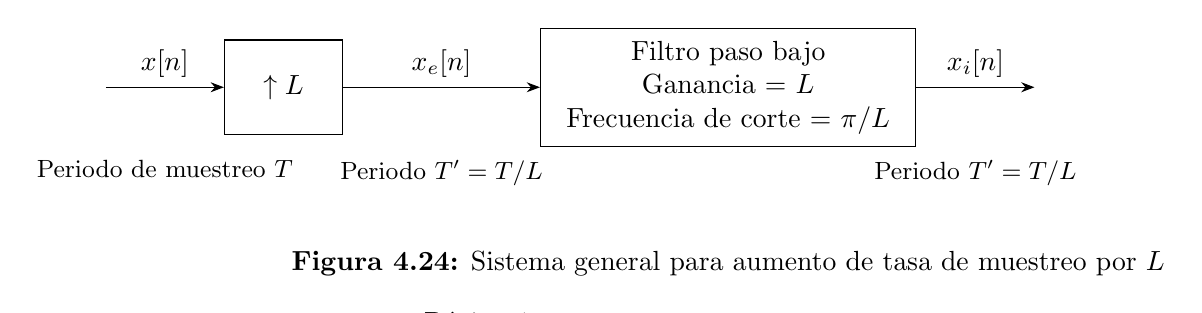
\begin{tikzpicture}[>=Stealth, auto, node distance=2.5cm]
  % Nodes
  \node [draw, minimum width=1.5cm, minimum height=1.2cm] (up) {$\uparrow L$};
  \node [draw, minimum width=3cm, minimum height=1.2cm, right=of up] (lpf) {\begin{tabular}{c}Filtro paso bajo\\Ganancia = $L$\\Frecuencia de corte = $\pi/L$\end{tabular}};
  
  % Input/Output
  \node [left=1.5cm of up] (input) {};
  \node [right=1.5cm of lpf] (output) {};
  
  % Arrows
  \draw[->] (input) -- node[above] {$x[n]$} node[below=0.8cm] {\small Periodo de muestreo $T$} (up);
  \draw[->] (up) -- node[above] {$x_e[n]$} node[below=0.8cm] {\small Periodo $T' = T/L$} (lpf);
  \draw[->] (lpf) -- node[above] {$x_i[n]$} node[below=0.8cm] {\small Periodo $T' = T/L$} (output);
  
  % Label
  \node [below=1.2cm of lpf] {\textbf{Figura 4.24:} Sistema general para aumento de tasa de muestreo por $L$};
\end{tikzpicture}
\end{center}

\vspace{0.5cm}

En este capítulo, hemos visto que el filtro paso bajo se puede implementar usando la DFT si el filtro es un filtro FIR de respuesta al impulso. Para este problema, suponga que este filtro tiene una respuesta al impulso $h[n]$ que es de $N+1$ puntos de longitud.

El siguiente diagrama muestra el sistema usando DFT, donde $H[k]$ es la DFT de $4N$ puntos de la respuesta al impulso del filtro paso bajo. Note que tanto $v[n]$ como $y[n]$ son secuencias de $4N$ puntos:

\begin{center}
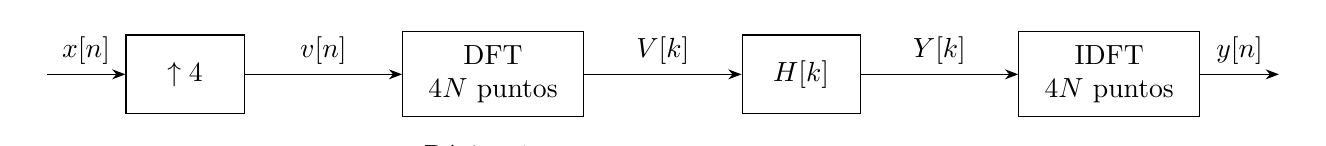
\begin{tikzpicture}[>=Stealth, auto, node distance=2cm]
  % Nodes
  \node [draw, minimum width=1.5cm, minimum height=1cm] (up) {$\uparrow 4$};
  \node [draw, minimum width=2cm, minimum height=1cm, right=of up] (dft) {\begin{tabular}{c}DFT\\$4N$ puntos\end{tabular}};
  \node [draw, minimum width=1.5cm, minimum height=1cm, right=of dft] (h) {$H[k]$};
  \node [draw, minimum width=2cm, minimum height=1cm, right=of h] (idft) {\begin{tabular}{c}IDFT\\$4N$ puntos\end{tabular}};
  
  % Input/Output
  \node [left=1cm of up] (input) {};
  \node [right=1cm of idft] (output) {};
  
  % Arrows
  \draw[->] (input) -- node {$x[n]$} (up);
  \draw[->] (up) -- node {$v[n]$} (dft);
  \draw[->] (dft) -- node {$V[k]$} (h);
  \draw[->] (h) -- node {$Y[k]$} (idft);
  \draw[->] (idft) -- node {$y[n]$} (output);
\end{tikzpicture}
\end{center}

\begin{parts}
  \part Especifique la DFT $H[k]$ tal que el sistema anterior implemente el sistema de sobremuestreo deseado. Piense cuidadosamente sobre la fase de los valores de $H[k]$.
  
  \part También es posible sobremuestrear $x[n]$ usando el siguiente sistema alternativo. Especifique el Sistema $A$ en la caja del medio de modo que la señal de $4N$ puntos $y_2[n]$ sea la misma que $y[n]$ del sistema anterior. Note que el Sistema $A$ puede consistir de más de una operación.
  
  \begin{center}
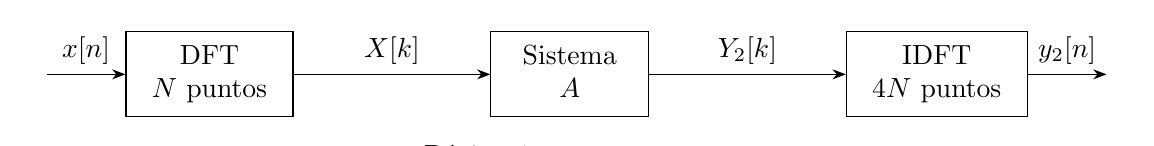
\begin{tikzpicture}[>=Stealth, auto, node distance=2.5cm]
  % Nodes
  \node [draw, minimum width=2cm, minimum height=1cm] (dft) {\begin{tabular}{c}DFT\\$N$ puntos\end{tabular}};
  \node [draw, minimum width=2cm, minimum height=1cm, right=of dft] (sysA) {\begin{tabular}{c}Sistema\\$A$\end{tabular}};
  \node [draw, minimum width=2cm, minimum height=1cm, right=of sysA] (idft) {\begin{tabular}{c}IDFT\\$4N$ puntos\end{tabular}};
  
  % Input/Output
  \node [left=1cm of dft] (input) {};
  \node [right=1cm of idft] (output) {};
  
  % Arrows
  \draw[->] (input) -- node {$x[n]$} (dft);
  \draw[->] (dft) -- node {$X[k]$} (sysA);
  \draw[->] (sysA) -- node {$Y_2[k]$} (idft);
  \draw[->] (idft) -- node {$y_2[n]$} (output);
\end{tikzpicture}
\end{center}
  
  \part ¿Existe una razón por la cual el sistema alternativo (parte b) podría ser preferible al primer sistema (parte a)?
\end{parts}

\end{questions}
\end{document}
\end{document}